\documentclass{article}
\usepackage{tikz}

\begin{document}

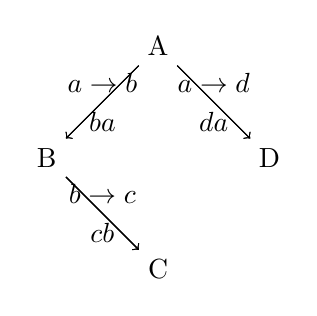
\begin{tikzpicture}[node distance=2cm]

% Define nodes for each summation method
\node (A) {A};
\node (B) [below left of=A] {B};
\node (C) [below right of=B] {C};
\node (D) [below right of=A] {D};

% Draw arrows to represent the relationships
\draw[->] (A) -- node[above] {$a \to b$} (B);
\draw[<-] (B) -- node[below] {$b \twoheadrightarrow a$} (A);

\draw[->] (B) -- node[above] {$b \to c$} (C);
\draw[<-] (C) -- node[below] {$c \twoheadrightarrow b$} (B);

\draw[->] (A) -- node[above] {$a \to d$} (D);
\draw[<-] (D) -- node[below] {$d \twoheadrightarrow a$} (A);

\end{tikzpicture}

\end{document}